\documentclass[12pt,a4paper,onecolumn]{scrartcl}
\usepackage[utf8]{inputenc}
\usepackage{amsmath}
\usepackage{amsfonts}
\usepackage{amssymb}
\usepackage[ngerman]{babel}
\usepackage[left=2.5cm,right=2.5cm,top=2.5cm,bottom=2.5cm,head=14.5pt]{geometry}
\usepackage{scrlayer-scrpage} % Zur Anpassung der Kopf- und Fußzeilen
\usepackage{graphicx}
\usepackage{float}
\usepackage{lmodern}
\usepackage{mathtools}
\usepackage{graphicx}
\usepackage{subfig}
\usepackage{caption, booktabs}
\usepackage{paralist}
\usepackage[toc,acronym,nonumberlist,translate=babel]{glossaries}
\usepackage{underscore}
\usepackage{float}
\usepackage{wrapfig}
\usepackage{array}
\usepackage{adjustbox}
\usepackage{makecell}
\usepackage{pdfpages}
\usepackage{csquotes}
\usepackage{hyperref}
\usepackage{chngcntr} % Damit Zählungen von Abb und Co innerhalb sections mögl
%\usepackage[scaled]{uarial} % Schriftart
\usepackage{url}

\usepackage[backend=biber,natbib=true,hyperref=true,
			style=draft,maxnames=2,maxbibnames=2, isbn=false]{biblatex}
% STYLE draft SPÄTER NOCH GEGEN authoryear TAUSCHEN!!!!!!
\addbibresource{literatur.bib} %% Einbinden der bib-Datei
\DefineBibliographyStrings{ngerman}{
	andothers = {{et\,al\adddot}},}

\def\theequation{\thesection.\arabic{equation}} % Formeln beginnen mit Abschnittssnummer
\linespread{1.0} % Zeilenabstand
\pagestyle{scrheadings}
\clearpairofpagestyles % Löschen der Platzhalter
\counterwithin{figure}{section} % damit figure je section neu gezählt werden

\newcommand*\mytitle{Arbeitstitel: Eisenhypothese Dust-Event 2009}
\newcommand*\mysubtitle{Bachelorarbeit}
\newcommand*\myauthor{Marco Schulz}
\newcommand*\mydate{05.03.2021}
\newcommand{\cotwo}{CO\textsubscript{2}}

\begin{document}
\begin{titlepage}
\begin{center}
{\LARGE \textsc{\mysubtitle}} \bigskip \\
{\huge \textsf{\mytitle}} \bigskip \\
{\Large \myauthor \ - Matrikelnummer 7345692} \smallskip \\
{\Large Fassung vom \mydate} \bigskip \\
\begin{figure}[H]
\centering

\includegraphics[width=60mm]{bilder/unilogo.png}
\end{figure}
\bigskip
{\Large Institut für Geophysik und Meteorologie}
\bigskip
{\Large \\ Universität zu Köln}
\vspace{4cm}
\\
\end{center}
\noindent Erstgutachter: Prof. Yaping Shao (yshao@meteo.uni-koeln.de)
\bigskip \\
Zweitgutachter: Prof. Joachim Saur (saur@geo.uni-koeln.de)
\end{titlepage}
\setcounter{page}{2}
\ofoot{\pagemark}
\chead{{\small \mytitle}}
\automark{section}
\tableofcontents
\newpage
\begin{abstract}
DIESEN QUATSCH HABE ICH MIT DEM IPAD GESCHRIEBEN
Das kann ich erst am Ende schreiben!
\end{abstract}
\section{Einleitung}
Klima verändert sich. Aktuell Eiszeitalter. Glaziale, Interglaziale abwechselnd. Bekannt (aus Eisbohrkernen), dass geringe \cotwo -Konzentration in Atmosphäre während Glazialen. Deckt sich mit den geringen Temperaturen. Wohin das ganze \cotwo ? Phytoplankton sorgt für $50\%$ des jährlichen \cotwo -Austauschs \citep{Field.1998} und erzeugen etwa 45 gt organischen Kohlenstoff pro Jahr \citep{Falkowski.1998}. Phytoplankton benötigt \cotwo \ zum Wachsen, wodurch dieses zu Biomasse konvertiert wird. Somit bei erhöhten Phytoplankton weniger \cotwo . Warum wächst Phytoplankton dann nicht beständig, bis alles \cotwo\ aufgebraucht? Weitere limitierende Faktoren, da zur Fotosynthese weitere Nährstoffe benötigt werden. Nitrat und Phosphate als Nährstoffe, auch von Tiefsee. \citet{Martin.1988} zeigen, dass Eisen limitierender Faktor. Eiseneintrag hauptsächlich aus Staub. Wenige Staubquellen in Südhemisphäre bzw. südl. Ozean (vgl. China/Sahara). Dadurch Eisenmangel, hingegen reich an Nitraten und Phosphaten aufgrund Upwelling (aufgrund Ekmantransport der zyklonalen Zirkumpolarströmung). Falls dann doch größere Eisendeposition, Phytoplankton-Blüten. Dies als mögliche Erklärung für geringe \cotwo - Konzentrationen während Glazialen (Modelle zeigen, dass dies ungefähr die Hälfte des \cotwo \ Rückgangs erklären könnte. Etwa 16 gt Kohlenstoff werden aktuell pro Jahr durch die biologische Pumpe im Ozean archiviert \citep{Falkowski.1998}. Wenn diese Hypothese angenommen, dann bei größeren Staub-Events (kleine Zeitskala) vermehrtes Phytoplankton Wachstum wahrscheinlich. Ein großes Event 2009 in Australien. Dieses soll in dieser Arbeit genauer untersucht werden. Abgleich Staub- bzw. Eisendeposition mit Entwicklung Phytoplankton (bzw. Chlorophyll-$\alpha$). Dazu benutze Kölner WRF-Staub-Weiterentwicklung. Vergleich mit Satellitenbildern. Nutze verschiedene Verfahren der Statistik. Berücksichtige Ozeanzirkulation und Wind. Falls Zusammenhang gezeigt werden kann dann Hypothese wahrscheinlich. Wäre weiteres Indiz für Eisenhypothese. Wurde schonmal gemacht \citep{Gabric.2016}. Prüfung des Kölner Modells. Zusammenhang $\Rightarrow$ ggf. ebenfalls Hinweis dass Modell gut.

\section{Theorie}
\subsection{Kohlendioxid und Klima}
\subsection{Wachstum von Phytoplankton}
Kurz: Welcher Prozess passiert genau bei Nährstoffe $\Rightarrow$ Phytoplankton / Fotosynthese \\\\
Phytoplankton sind Einzeller.
Wachstumsbeeinflussende Faktoren sind \citep{Falkowski.1998}):
\begin{enumerate}
\item mixed-layer depth
\item nutrient fluxes
\item food-web structure
\end{enumerate}
\citet{Boyce.2010} folgern, dass der Reichtum an Phytoplankton insgesamt seit Beginn der Messungen (1899) aufgrund der Erwärmung der Ozeane abgenommen hat. Es wird geschätzt, dass das globale Median jährlich um etwa 1\% abnimmt. Da die Klimamodelle steigende (Meeres-)Temperaturen prognostizieren ist es wahrscheinlich und problematisch, dass die Menge an Phytoplankton, der Basis aller Nahrungsketten im Ozean, zukünftig noch weiter abnimmt \citep{Siegel.2010}. Klimaänderungen werden direkt (andere Ozeanchemie) und indirekt (Änderungen in der Ozeanzirkulation) die Verteilung des Phytoplanktons verändern \citep{Falkowski.1998}.

\subsection{Eisenhypothese}
Andere Nährstoffe für Phytoplankton können durch aufsteigendes Tiefenwasser bereitgestellt werden. Eisen und Mangan werden hingegen hauptsächlich durch äolischen Staub eingebracht. Verweildauer von etwa 6 Monaten in oberflächennahem Wasser bis ca. 150m Tiefe
\citep{Hayes.2015}. Insbesondere im südlichen Ozean kann auch Mangan limitierender Faktor sein \citep{Browning.2021}.
\begin{figure}[ht]
\centering
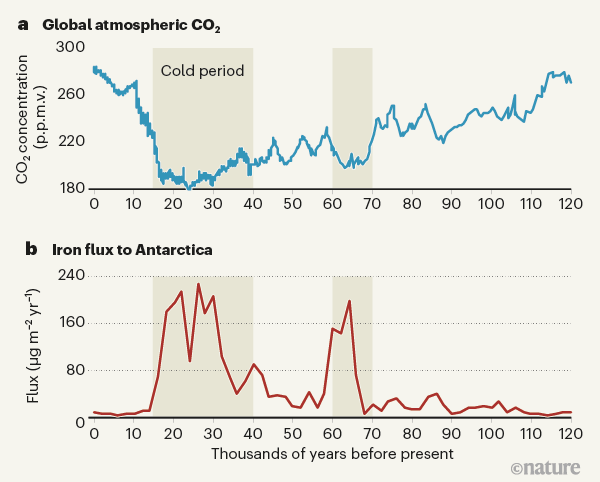
\includegraphics[width=0.7\textwidth]{bilder/Stoll2020/antarctic-iron-global-co2.png}
\caption{Antikorrelation von \textbf{a} globaler \cotwo \ Konzentration und \textbf{b} Eisendeposition in der Antarktis \citep{Stoll.2020}}
\end{figure}
\subsubsection{Düngung funktioniert nicht}
verschiedene Ursachen. Verweilzeit in Oberflächenwasser \citep{Hayes.2015}. Aufnahmefähigkeit / Rezeptivität ist saisonal variabel \citep{Gabric.2016}, Sekundärquelle
\subsubsection{Biologische Pumpe}
Niedriger Sauerstoffgehalt in der Tiefsee weist auf starke biologische Pumpe hin (dortige durch mehr absinkendes Plankton angereicherte Organismen verbrauchen mehr Sauerstoff)

\subsection{Staubkreislauf}
wichtige Verbindung zu Energie- und Kohlenstoffkreislauf \citep{Shao.2011}
\subsubsection{Staubquellen in Australien}
größte Teil Zentralaustralien \citep{Shao.2011} siehe auch Lake Eyre basin
\subsubsection{Eisen in Staub}
Nicht jede Form von Eisen kann als Dünger dienen. Muss entsprechend gelöstes (?) Eisen sein. Transportprozesse und Wolkenbildungen können die Transformation zu diesem tauglichen Eisen fördern \citep{Shao.2011}. Die Planktonart Trichodesmium kann die Rate des Eisenauflösens von Oxiden und Staub beschleunigen (im Gegensatz zu anderem Phytoplankton) \citep{Gabric.2016}
\subsubsection{Emissions- und Depositionsmodelle}
ggf. lieber in Kapitel Methoden
\subsection{Wind und Oberflächenströmungen}
Verkleinerung der Tiefe der Oceanic Mixed Layer von September auf Oktober \citep{Tilburg.2002} (abchecken, dass der Bloom nicht daher kommt!). Einteilung in \textit{nördlich der Tasmanischen Front} und \textit{südlich der tasmanischen Front}? Phytoplanktonproduktion hängt von Up- und downwelling-Prozessen durch mesoskalige Wirbel ab \citep{Tilburg.2002}
\subsection{Dust-Event Australien 2009}




\section{Methoden}
hole Zeitreihe Chlorophyll alpha Entwicklung von September bis Oktober (bzw. falls saisonale Veränderung, den Zeitraum, welcher der Kurve Dust-Event-Zeitraums entspricht) gemittelt über bspw. 10 Jahre. Berechne daraus Anomalie 2009 und vergleiche diese mit Staubdeposition.
\subsection{iron residence time modell}
\subsection{phytoplankton response time modell}
turn-over time ist von Größenordnung einer Woche oder weniger \citep{Falkowski.1998}.

\subsection{WRF Modell}
nur kurze Vorstellung, da grundsätzlich nur der Output verwendet werden soll. Vergleich mit von \cite{Gabric.2016} genutzem Modell CEMSYS
\subsection{Phytoplankton}
Climate Data Store \nocite{*}
\\\\
Messungen des Chlorphyll-$\alpha$ geben Rückschluss auf Phytoplankton \citep{RYTHER.1957}(muss ich noch lesen)

\subsection{EOF?}
\subsection{Riegers Principal Components?}

\section{Auswertung und Diskussion}
\section{Zusammenfassung und Ausblick}
\newpage
\printbibliography
\newpage
\appendix
\section{Anhang}
\addcontentsline{toc}{section}{Abbildungsverzeichnis}
\listoffigures
\addcontentsline{toc}{section}{Tabellenverzeichnis}
\listoftables
\section{Danksagung}
\end{document}
